% =============================================================================
% Section 7. The opportunity-security space
% Inputs: energy_security_index, economic_opportunity_index and their category and variable
% contributions (scripts/20_build_indices.R); the Strategic Index of Section 8 (eq:si).
% Results: paper/results/joint.json, scripts/paper/fig_joint.R (final rerun of 2026-10-12).
% Postures: RMI (2025) as labelled in config/country_insights.yml (quadrants) and
% R/charts/Country_Sector_Megatable.R (derive_strategic_path). Further results: Online Appendix
% (sections/oa_joint.tex, oa:joint).
% =============================================================================
\section{The opportunity-security space}\label{sec:joint}\label{sec:joint_space}

Each country-technology-stage cell is a point $(\ES_{its},\EO_{its})$ of the unit square. The
Strategic Index of Section~\ref{sec:strategic} reads the two pillars together, and its pillar terms
in equation~\eqref{eq:si} carry equal weights of opposite sign, so they reduce to the gap between
opportunity and security:
\begin{equation}\label{eq:joint_gap}
  0.3\,\EO_{its}+0.3\,(1-\ES_{its})=0.3+0.3\,\Delta_{its},\qquad
  \Delta_{its}\equiv\EO_{its}-\ES_{its}.
\end{equation}
The index favours cells in which opportunity exceeds security, and treats alike a cell that is
secure and well placed and one that is neither. Because it ranks a country's own sectors, what
matters is how $\Delta_{its}$ varies across them:
\begin{equation}\label{eq:joint_var}
  \operatorname{Var}_i(\Delta)=\operatorname{Var}_i(\EO)+\operatorname{Var}_i(\ES)
  -2\operatorname{Cov}_i(\EO,\ES).
\end{equation}
If the pillars rise together across a country's sectors, the gap is compressed and the policy term
and sector priors move the ranking more than their nominal weights suggest
\citep{paruolo2013ratings,becker2017weights}.

Part of the association is built in. Four categories enter both pillars with identical values, and
Trade and Foreign Dependency share components (Table~\ref{tab:shared_signals}). By the variable
decomposition of equation~\eqref{eq:var_decomp}, each pillar splits into the contribution of the
shared components and of the rest, $P_{its}=A^{P}_{its}+B^{P}_{its}$, and for any set of cells
\begin{equation}\label{eq:joint_cov}
  \operatorname{Cov}(\ES,\EO)=\operatorname{Cov}(A^{\ES},A^{\EO})
  +\operatorname{Cov}(A^{\ES},B^{\EO})+\operatorname{Cov}(B^{\ES},A^{\EO})
  +\operatorname{Cov}(B^{\ES},B^{\EO}).
\end{equation}
With fixed weights the first term is a positively weighted sum of the covariances of the shared
components: it records construction, not an economic link. In the gap those components enter with
coefficients $\omega^{\EO}\lambda^{\EO}-\omega^{\ES}\lambda^{\ES}$ and partly cancel
(equation~\eqref{eq:eo_si_shared}), so the information on where the gap is large lies mainly in
$B^{\ES}$ and $B^{\EO}$.

We report within-pair rank correlations from the full pillars and from $B^{\ES}$ and $B^{\EO}$
alone, and classify cells by each pillar's position relative to its within-pair median. The four
regions correspond to the four strategic postures of \citet{carey2025secure}, which read the same
two-dimensional space, in the labelling of the dashboard built on these indices: opportunity without security
(leapfrog: build capability), leaders (export promotion), laggards (friendshore: secure supply
through partners, the case of Sections~\ref{sec:bilateral} and~\ref{sec:network}) and security
without opportunity (alternative value creation). The correspondence is a reading aid, with the
median of each pair as the cut. As \citet{neis2026allied} stresses, security risk and economic
opportunity are not synonyms, and the same exposure can warrant different postures; the results
below measure how far the two pillars carry distinct information.

\subsection{Results}\label{subsec:joint_results}

\paragraph{Sample and co-movement.} Both pillars score 6{,}232 cells; 3{,}157 cells for 175
economies in 30 pairs are rankable on both (607 territory cells and 2{,}468 sovereign cells over
the imputation threshold are set aside), among them 1{,}500 cells of the 57 coalition members. The
median within-pair Spearman correlation of $\ES_{its}$ and $\EO_{its}$ is 0.59 (interquartile range
0.45 to 0.77), from $-0.21$ in Green Hydrogen midstream to 0.94 in Electric Vehicles midstream
(Table~\ref{tab:joint_stage}). It rises along the chain: 0.44 upstream, 0.58 midstream and 0.78
downstream (Figure~\ref{fig:joint_scatter}), a gradient that also holds within most technologies.

\begin{figure}[tbp]
  \centering
  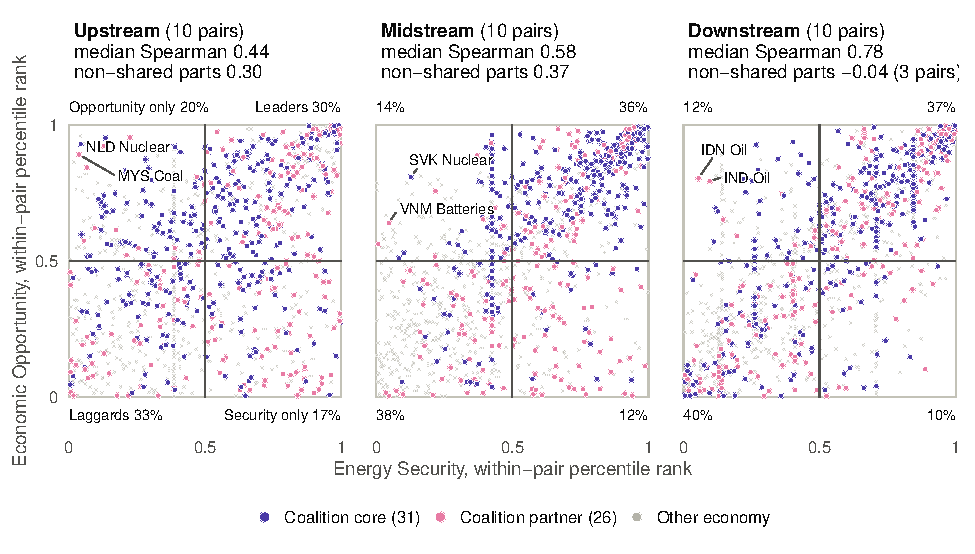
\includegraphics[width=\textwidth]{joint_scatter}
  \caption{The opportunity-security space. Each point is a cell rankable on both pillars, at its
  within-pair percentile rank on $\ES_{its}$ (horizontal) and $\EO_{its}$ (vertical); panels are
  stages. Violet: the 31 core members; pink: the 26 partners; gray: other economies. Lines at 0.5
  mark the within-pair medians and divide the regions (a cell at the median counts as low); corner
  percentages are the stage's shares. Panel headers give the median within-pair Spearman
  correlation from the full pillars and from the non-shared parts $B^{\ES}$, $B^{\EO}$ of
  equation~\eqref{eq:joint_cov}. The dense column left of the upstream security median is Nuclear
  upstream, where 87 of 175 economies without uranium share $\ES_{its}=0.172$. Sample: 3{,}157 cells,
  175 economies, 30 pairs. Source: \texttt{index\_outputs.rds}; \texttt{scripts/paper/fig\_joint.R}.}
  \label{fig:joint_scatter}
\end{figure}

\paragraph{How much is mechanical.} Shared components carry 61 per cent of the effective weight of
$\ES_{its}$ (25, 62 and 91 per cent by stage) but 28 per cent of that of $\EO_{its}$; in seven
downstream pairs every security component also enters opportunity. On the 23 pairs where both
pillars keep components of their own, the median correlation falls from 0.55 to 0.30 when only
non-shared components are used. The shared term accounts for 61 per cent of the pooled within-pair
covariance (7, 42 and 87 per cent by stage). What remains runs mainly through trade: the
largest cross-pillar category correlation is between security's Minerals Trade and opportunity's
Trade (0.76), while Technology Demand and Cost Competitiveness are nearly orthogonal to every
security category (Figure~\ref{fig:joint_corr}). Net of shared inputs, security and opportunity
are close to unrelated across economies except where exports reveal both.

% Generated by scripts/paper/fig_joint.R; do not edit by hand.
\begin{table}[tbp]
\centering
\begin{threeparttable}
\caption{Energy Security and Economic Opportunity within technology-stage pairs, by stage}
\label{tab:joint_stage}
\footnotesize
\begin{tabular}{@{}lcccc@{}}
\toprule
 & Upstream & Midstream & Downstream & All \\
\midrule
Technology-stage pairs & 10 & 10 & 10 & 30 \\
Country cells & 999 & 1,048 & 1,110 & 3,157 \\
\addlinespace
\multicolumn{5}{@{}l}{\textit{Spearman correlation of $\ES_{its}$ and $\EO_{its}$ within pairs}}\\
\quad Median across pairs & 0.44 & 0.58 & 0.78 & 0.59 \\
\quad Lowest pair & 0.03 & $-$0.21 & 0.40 & $-$0.21 \\
\quad Highest pair & 0.63 & 0.94 & 0.92 & 0.94 \\
\quad Pooled within-pair ranks & 0.39 & 0.60 & 0.71 & 0.57 \\
\addlinespace
\multicolumn{5}{@{}l}{\textit{Components shared by the two pillars}}\\
\quad Effective weight in $\ES$ & 0.25 & 0.62 & 0.91 & 0.61 \\
\quad Effective weight in $\EO$ & 0.26 & 0.20 & 0.37 & 0.28 \\
\quad Pairs with both non-shared pillars defined & 10 & 10 & 3 & 23 \\
\quad Median correlation, non-shared pillars & 0.30 & 0.37 & $-$0.04 & 0.30 \\
\quad Median correlation, full pillars, same pairs & 0.44 & 0.58 & 0.58 & 0.55 \\
\quad Share of level covariance, shared term & 0.07 & 0.42 & 0.87 & 0.61 \\
\quad Share of level covariance, non-shared term & 0.58 & 0.20 & 0.00 & 0.16 \\
\addlinespace
\multicolumn{5}{@{}l}{\textit{Share of cells by region of the space (percent)}}\\
\quad Opportunity without security & 19.5 & 13.8 & 12.4 & 15.1 \\
\quad Leaders (both high) & 30.2 & 36.0 & 37.2 & 34.6 \\
\quad Security without opportunity & 17.2 & 12.5 & 10.2 & 13.2 \\
\quad Laggards (both low) & 33.0 & 37.7 & 40.2 & 37.1 \\
\bottomrule
\end{tabular}
\begin{tablenotes}[flushleft]\footnotesize
\item \textit{Notes:} Eleven headline technologies; cells rankable on both pillars only (a sovereign economy with at most half of the pillar's weight imputed), which leaves 3,157 of the 6,232 cells that both pillars score, for 175 economies. A technology-stage pair enters when both pillars score it and neither pillar's diagnostics flag it as constant or unscored, which leaves 30 of the 33 pairs: Energy Security does not score downstream grid or upstream and midstream geothermal. Correlations are Spearman correlations across economies within a pair; the pooled row is the Pearson correlation of within-pair percentile ranks over all cells of the stage. A component is shared when the other pillar contains a component of the same category with identical observed values; its effective weight is its category weight times its within-category weight, averaged over cells. Non-shared pillars are the weighted means of the remaining components with the weights renormalised; they are undefined where every component of $\ES$ is shared, as in 7 downstream pairs, and the last two correlation rows use only the pairs in which both are defined. The covariance shares decompose the within-pair covariance of the pillar levels as in equation~\eqref{eq:joint_cov}, pooled over pairs with weights $n-1$: the shared term is $\operatorname{Cov}(A^{\ES},A^{\EO})$, the non-shared term $\operatorname{Cov}(B^{\ES},B^{\EO})$, and the two cross terms make up the remainder. Regions are defined by the within-pair medians of the two pillars, a cell at the median counting as low. Source: \texttt{index\_outputs.rds}; \texttt{scripts/paper/fig\_joint.R}.
\end{tablenotes}
\end{threeparttable}
\end{table}


\begin{figure}[tbp]
  \centering
  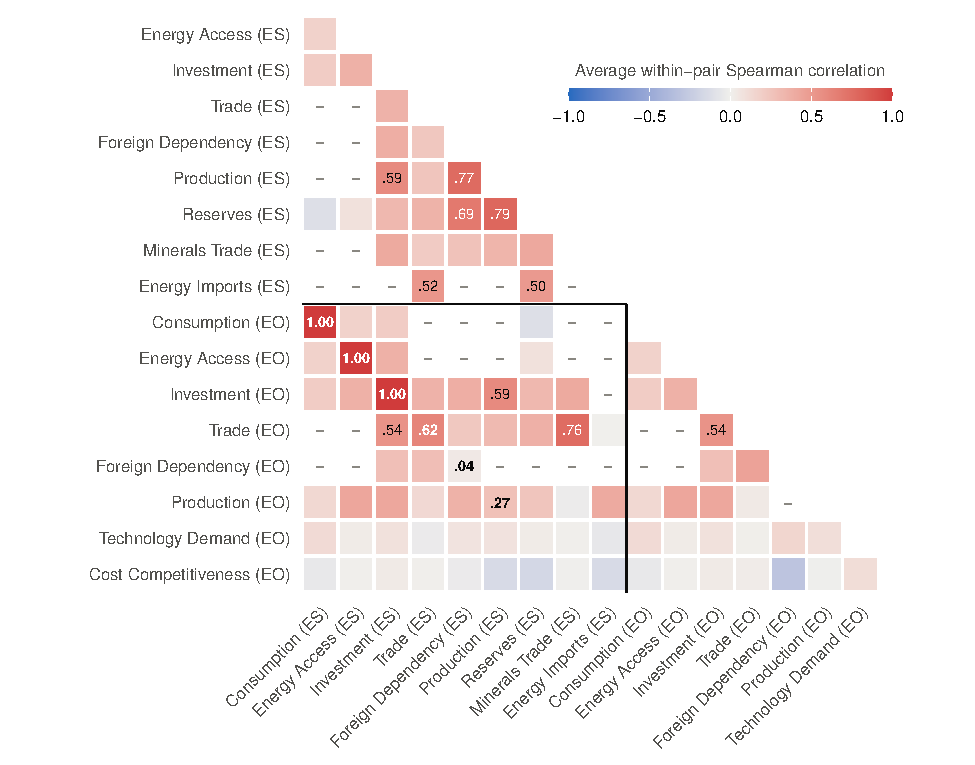
\includegraphics[width=\textwidth]{joint_corr}
  \caption{Average within-pair Spearman correlation between the categories of the two pillars
  (pairs with at least 20 rankable economies in which both categories vary). The black lines
  separate the cross-pillar block (bottom left) from the within-pillar blocks; bold numbers mark
  categories entering both pillars under the same name. Energy Prices and Technological Readiness,
  constant within every pair, are omitted. Sample: as Figure~\ref{fig:joint_scatter}. Source:
  category scores in \texttt{index\_outputs.rds}; \texttt{scripts/paper/fig\_joint.R}.}
  \label{fig:joint_corr}
\end{figure}

\paragraph{Regions.} Pooling all pairs, 15.1 per cent of cells have opportunity without security,
34.6 per cent are leaders, 13.2 per cent have security without opportunity and 37.1 per cent are
laggards (12.6, 37.7, 15.3 and 34.4 per cent if ties count as high). The shares largely restate the
rank correlation: a Gaussian copula with each pair's correlation implies an off-diagonal share of
14.6 per cent, against 14.2 observed. Opportunity without security is most common upstream (19.5
per cent), where the pillars are least related. The largest pair shares, Green Hydrogen midstream
(45 per cent) and Nuclear upstream (28), are tie artefacts (Figure~\ref{fig:joint_quadrants});
without them the pooled share is 14.0 per cent.

\begin{figure}[tbp]
  \centering
  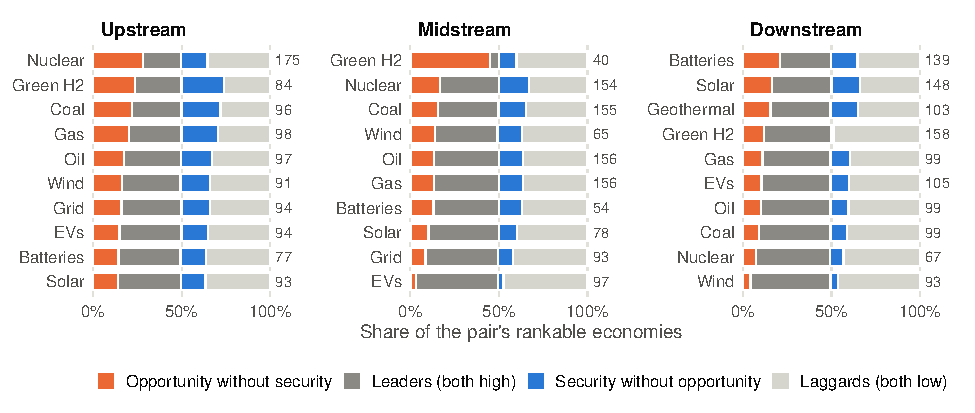
\includegraphics[width=\textwidth]{joint_quadrants}
  \caption{Shares of each pair's rankable economies in the four regions of
  Figure~\ref{fig:joint_scatter}, by stage, ordered by the share with opportunity but not security
  (orange); blue marks security without opportunity, dark gray leaders, light gray laggards. The
  two longest orange segments are ties at the security median: in Green Hydrogen midstream 34 of
  40 economies share the lowest $\ES_{its}$, and in Nuclear upstream 87 of 175 share the median
  value. Source: as Figure~\ref{fig:joint_scatter}.}
  \label{fig:joint_quadrants}
\end{figure}

\paragraph{The coalition.} Of the members' cells, 49.3 per cent are leaders and 12.8 per cent have
opportunity without security (core 55.1 and 16.4 per cent, partners 40.4 and 7.4;
Figure~\ref{fig:joint_members}), partly because scale raises both pillars; the United States is a
leader in 29 of 30 pairs. Austria, Portugal and Luxembourg have the most leapfrog-type pairs (11 of
30 each); Brazil (19 of 29), Peru and T\"urkiye have the most security without opportunity.

\begin{figure}[tbp]
  \centering
  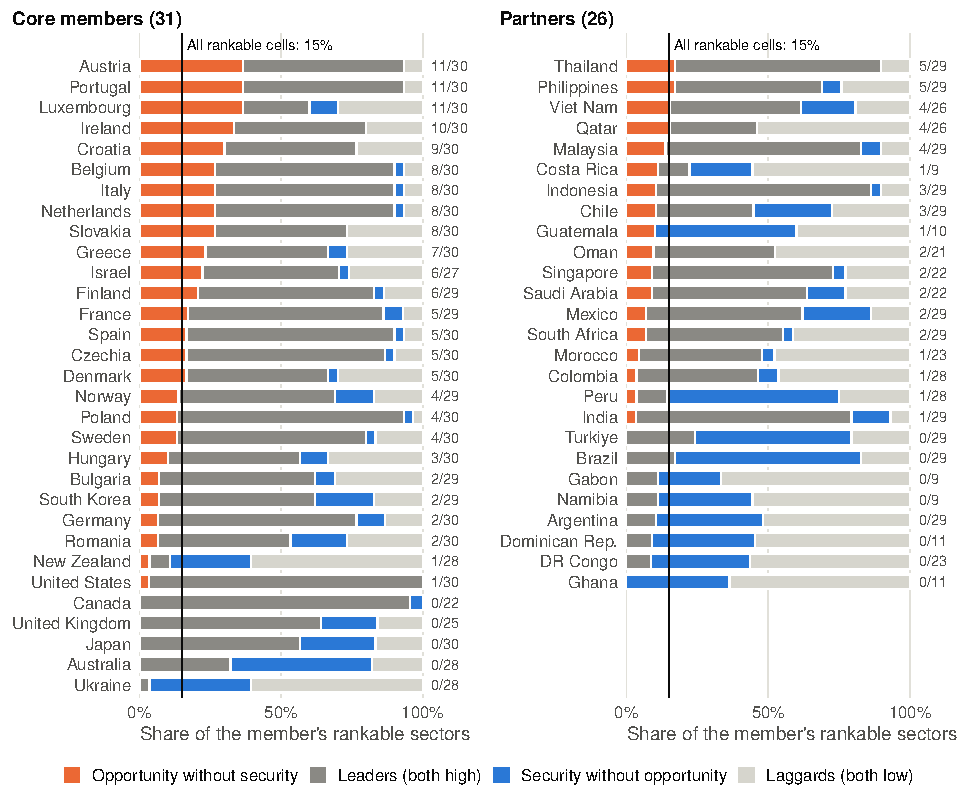
\includegraphics[width=\textwidth]{joint_members}
  \caption{Each coalition member's rankable pairs divided among the four regions: the 31 core
  members (left) and 26 partners (right), ordered by the share with opportunity but not security;
  the fraction gives that count over the member's rankable pairs (9 to 30). The vertical line is
  the all-cell share (15 per cent). Nuclear upstream and Green Hydrogen midstream account for 25 of
  the 192 member pairs in orange. Source: as Figure~\ref{fig:joint_scatter}.}
  \label{fig:joint_members}
\end{figure}

\paragraph{Within countries and the Strategic Index.} Across the sectors of each of the 167
countries with at least five Strategic Index cells, the correlation of $\EO_{its}$ and $\ES_{its}$
averages 0.46 (from $-0.56$ to 0.84), and the covariance term removes on average 36 per cent of
$\operatorname{Var}_i(\EO)+\operatorname{Var}_i(\ES)$ (42 per cent for members), leaving a standard
deviation of $\Delta_{its}$ of 0.13. The index does favour the leapfrog region (mean 0.563 there,
against 0.511 to 0.545 elsewhere), and 8 of the 57 allied picks lie in it (14.0 per cent, against
6.7 per cent of eligible sectors). Four of the nine Nuclear midstream picks come from small
partners with four or five eligible sectors; their security ranks lie at or above a compressed
median, so the picks reflect the technology weight of equation~\eqref{eq:si} (0.999 for nuclear
against 0.42 for gas), not a security floor. Across a country's sectors the index correlates 0.63
with the level gap but only 0.19 with the gap in within-pair ranks: it reflects which pairs score
high opportunity and low security for everyone at least as much as where the country stands.
Online Appendix~\ref{oa:joint} gives further detail and caveats.
